\section{Single cooper pair box system\label{sec:cooper_pair_box}}
\begin{figure}[h]
  \centering \includegraphics[height=5cm]{energy_ratios_for_qubit}
  \caption{\small       General        overview       of       energy
    parameters\label{fig:energy_ratios_for_qubit}}
\end{figure}

\begin{enumerate}
\item   Starting  with   \autoref{fig:cooper_pair_box_1_no_gate}  and
  remembering   Faraday's  law   ($V  =   -\dot{\Phi}$),  we   read  the
  \textbf{charging  kinetic part},  that  comes as  a  result of  the
  time-varying flux on the cooper pair island.

  \begin{equation}
    T = \frac{C_g}{2}\dot{\Phi_J}^2 + \frac{C_J}{2}\dot{\Phi_J}^2 = \frac{C_\Sigma}{2}\dot{\Phi_J}^2.
  \end{equation}

  \begin{figure}[h]
    \centering \inkfig{6cm}{cooper_pair_box_1_no_gate}
    \caption{\small The Cooper pairs are trapped on an island between
      a       gated       capacitor       and       a       Josephson
      junction.\label{fig:cooper_pair_box_1_no_gate}}
  \end{figure}

\item \textbf{The potential  energy part} comes from the  JJs and the
  energy of  the gate  voltage acting  on the  induced charge  on the
  capacitor.

  \begin{equation}
    \left\{
      \begin{aligned}
        & E_J = 1 - E_J\cos(\frac{2\pi}{\Phi_0}\Phi_J)\\
        &  \begin{aligned} E_\text{gate}  & =  V_g \times  Q_g\\b Q_g  & =
          C_g\times -\dot{\Phi_J}b
        \end{aligned}
      \end{aligned}\right.  \rightarrow U =
    -E_J\cos(\frac{2\pi}{\Phi_0}\Phi_J)
    -
    V_gC_g\dot{\Phi_J}.
  \end{equation}

  \begin{figure}[h]
    \centering \inkfig{8cm}{cooper_pair_box_2_with_gate}
    \caption{\small            Addition            of            bias
      voltage\label{fig:cooper_pair_box_2_with_gate}}
  \end{figure}

\item The full \textbf{Lagrangian} now reads
  \begin{equation}
    \mathcal{L} = T - U = \frac{C_\Sigma}{2}\dot{\Phi}_J^2 + E_J\cos\left( \frac{2\pi}{\Phi_0}\Phi_J \right) + V_gC_g\dot{\Phi_J}.
  \end{equation}

\item  The \textbf{conjugate  momentum},  which gives  useful set  of
  generalised coordinates to work with,

  \begin{equation}
    Q_J = \frac{d\mathcal{L}}{d\dot{\Phi}_J} = \slate{C_\Sigma\dot{\Phi}_J} + \gold{V_gC_g},
  \end{equation}
  \noindent turns out to be  the \slate{\textbf{induced charge on the
      capacitor   due   to   the   JJ   voltage}}   offset   by   the
  \gold{\textbf{charge induced by the gate voltage $V_g$}}.

\item So we arrive at the following set of variables

  \begin{equation}
    { \textcolor{blue}{\mathbf{x\leftrightarrow \Phi \leftrightarrow \phi} \text{ (position/flux) }}\qquad \textcolor{red}{\mathbf{p\leftrightarrow Q \leftrightarrow N \text{ (momentum/electrons) }}}}
  \end{equation}

  \noindent with the commutation relations:

  \begin{align}
    \left[\blue{x},\red{p}\right] & =i\hbar & \left[\blue{\Phi},\red{Q}\right] & = i\hbar & \left[\phi,N\right] & = \frac{2\pi}{\frac{h}{2e}}\left[\Phi,Q\right]\frac{1}{2e} = i\\
    \red{\hat{p}} & = -i\hbar\ipartial{}{\blue{x}} & \hat{\red{Q}} & =-i\hbar\ipartial{}{\blue{\Phi}} & \hat{\red{N}} & =-i\ipartial{}{\blue{\phi}}
  \end{align}

\item\

\begin{framed}\noindent
  The Hamiltonian is then:

  \begin{equation}\label{eqn:cpbox_final}
    \begin{aligned}
      \mathcal{H} & = Q_J\dot{\Phi}_J - \mathcal{L}\\
      & = \frac{(Q_J - C_gV_g)^2}{2C_\Sigma} - E_J\cos(\frac{2\pi}{\Phi_0}\Phi_J)\\
      &   =   \mathbf{\red{4E_C{\left(\hat{N}-N_\text{ext}\right)^2}-
          E_J\cos\left(\phi\right)}}\qquad E_c = \frac{e^2}{2C_\Sigma}
    \end{aligned}
  \end{equation}

  \noindent We  will call $  N_\text{ext} = \frac{C_g V_g}{2e}  $ the
  effective offset charge and $C_{\Sigma} = C_g+C_J$.
\end{framed}
\end{enumerate}

\subsection{Adding a parallel JJ\label{subsec:cpb_2}}
\begin{framed}\noindent
  A parallel JJ  will allow one to  tune the energy of  the system by
  varying the biasing magnetic field.
\end{framed}

\begin{figure}[h]
  \centering \inkfig{8cm}{cooper_pair_box_3_tuneable}
  \caption{\small Adding a  sencond JJ will allow one  to control the
    effective   energy   $E_{J}$  and   thus   the   energy  of   the
    system.\label{fig:cooper_pair_box_3_tuneable}}
\end{figure}

\begin{itemize}
\item  The   two  currents   through  the  JJ   will  give   a  total
  current \begin{equation} I = I_{c1}\sin(\phi_1)+I_{c2}\sin(\phi_2),
  \end{equation}

\item               The              phase               quantisation
  ($ \phi_1-\phi_2 = \phi_\text{ext} + 2\pi  m, m \in \mathbb{Z} $) and
  symmetric JJs ($I_{c1}=I_{c2}=I_{c0}$) results in

  \begin{equation}
    \begin{aligned}
      I & = 2I_{c0}\sin(\frac{\phi_1+\phi_2}{2})\cos(\frac{\phi_1-\phi_2}{2})) \\
      &                                                             =
      2I_{c0}\cos(2\pi\frac{\Phi_{\text{ext}}}{2\Phi_0})\sin(\frac{\phi_1+\phi_2}{2})
    \end{aligned}
  \end{equation}

\begin{framed}\noindent
  In effect, the two JJ acts as a single JJ with current
  \begin{equation}
    I = \slate{I_{c}}\sin(\gold{\phi})
  \end{equation}
  \noindent    where   the    critical    current,    $I_c$   is    a
  magnetic-field-controlled parameter.
  \begin{equation}
    \slate{I_{c}(\Phi_\text{ext}) = 2I_{c0}|\cos(\pi\Phi_\text{ext}/\Phi_0)|} \qquad \gold{\phi = (\phi_1+\phi_2)/2}
  \end{equation}

\end{framed}

\item   The  potential   energy  $U(\Phi_{\text{ext}})$   is  now   a
  field-controlled parameter:

  \begin{equation}
    \left\{\begin{aligned}
        I &= \slate{I_c(\Phi_\text{ext})}\sin(\phi)\\
        V&=\dot{\Phi} \equiv \frac{\dot{\phi}}{2\pi}\Phi_0
      \end{aligned}\right.  \Rightarrow U =
    \left\{
      \begin{aligned}
        \int_{0}^{t}IV dt & = \int_{0}^{t}\slate{I_c(\Phi_\text{ext})}\sin(\phi)\frac{\Phi_0}{2\pi}\frac{d\phi}{dt}dt\\
        & = \int_{0}^{\phi} E_J\sin(\phi)d\phi\\
        &      =      \red{E_J}(1-\cos(\phi))     \qquad      \red{E_J      =
          \ballblue{\frac{\Phi_0I_{c0}}{2\pi}}                      \times
          2|\cos(\pi\Phi_\text{ext}/\Phi_0)|}.
      \end{aligned}\right.
  \end{equation}
  \begin{framed}\noindent
    Thus  the  Josephson energy  from  the  JJ elements  acquires  an
    additional factor which can now be controlled:
    \begin{equation}
      E_J = \ballblue{E_{J0}} \times 2|\cos(\pi\Phi_\text{ext}/\Phi_0)|
    \end{equation}
  \end{framed}
\end{itemize}

\subsection{Transmon}
\label{sec:transmon}

A  transmon  extends the  cooper  pair  box,  by boosting  the  ratio
$\frac{E_{J}}{E_{C}}$.   This  is  done by  decreasing  the  charging
energy  $E_c= \frac{e^2}{2C_\Sigma}$  by  introducing  a large  shunt
capacitance in parallel to the JJs.

\begin{framed}\noindent
  \begin{equation}
    C_{\Sigma} =  \gold{\mathbf{C_\text{transmon}}} + C_g  + C_J.
  \end{equation}
\end{framed}

\begin{figure}[h]
  \centering \inkfig{7cm}{cooper_pair_box_4_transmon}
  \caption{\small  Transmon suppresses  $E_{C}$  with  a large  shunt
    capacitance. \label{fig:cooper_pair_box_4_transmon}}
\end{figure}

\newpage
\begin{framed}\noindent
  \textbf{Summarising up to now}:
  \begin{equation}\label{eq:cooper-pair-box-summary}
    \begin{aligned}
      \mathcal{H} & = 4E_C{\left(\hat{N}-N_\text{ext}\right)^2} -
      E_J(\Phi_{\text{ext}})\cos\left(\phi\right)\\
      E_c& = \frac{e^2}{2C_\Sigma}\\
      N_\text{ext} & = \frac{C_g V_g}{2e} && \text{Induced charge from the gate}\\
      C_{\Sigma} & = \blue{C_\text{transmon} + C_g}+ \green{C_J}\\
      E_J(\Phi_{\text{ext}}) & = \ballblue{E_{J0}} \times 2|\cos(\pi\Phi_\text{ext}/\Phi_0)| && \text{controlled by the applied external flux}.\\
    \end{aligned}
  \end{equation}

  \subsubsection{Capacitance through parallel structures}
  \label{sec:capac-thro-parall}
  As    stated     in    Sec.~\ref{sec:coupling-capacitance},    each
  \iunit{10}{$\mu$m} of parallel structures  adds on \iunit{1}{fF} of
  capacitance ($10^{-10}\,$F/\mum).
  \begin{equation}
    \blue{C_{g} \text{ or } C_{\text{transmon}} = \iunit{1}{fF} \times \text{per 10$\mu$m of interface}}.
  \end{equation}

\begin{center}
  \inkfig{8cm}{capacitances_through_parallel_structures}
\end{center}

\subsubsection{Capacitances from JJ}
\label{sec:capacitances-from-jj}
\begin{itemize}
\item The JJ (see below) act like capacitors due to the Al0$_x$ oxide
  layer between them:
  \begin{equation}
    \green{C_J = \frac{\varepsilon\varepsilon_0A_{JJ}}{d}}
  \end{equation}
  \noindent  where   $A_{JJ}$  is  the   contact  area  of   the  JJ,
  \iunit{d=2}{nm}, $\varepsilon = 10$.

  \red{\textbf{This  contribution will  be relatively  small for  the
      Transmon.}}
\end{itemize}

\subsection{The critical current and $E_{J0}$}
\label{sec:crit-curr-josephs}

  \begin{equation}
    I_cR_n      =
    \frac{\pi\Delta(T)}{2e}\tanh\big(\frac{\Delta(T)}{2k_bT}\big)
  \end{equation}

  \noindent     can     derived      from     BCS     theory     (see
  Eq.\eqref{introducing-qed-operators-critical-current})     for    a
  superconducting  energy  gap of  $  \Delta(T)  $ and  normal  resistance
  $  R_n   $  of  the   JJ,  which  in  the   limit  $T  \rightarrow   0$  read
  $ I_cR_n = \frac{\pi\Delta(0)}{2e}$ so that
  \begin{equation}
    \ballblue{E_{J0} = \Phi_0I_c\frac{1}{2\pi} = \frac{h}{2e}\frac{\pi\Delta(0)}{2eR_n}\frac{1}{2\pi} \equiv \frac{R_q}{R_{\square}/N_{sq}}\frac{\Delta(0)}{2}}
  \end{equation}

  \noindent where

  \begin{itemize}
  \item $R_{q} = \frac{h}{(2e)^{2}}$;
  \item  $R_n =  R_{\square}/ N_{\text{sq}}$  is the  resistance of  the JJ
    oxide  layer.   The  more  \iunit{100  \times  100}{nm$^{2}$}  squares
    ($N_{\text{sq}}$), the lower the resistance.

     \begin{equation}
       R_{\square} = 1.84\,\text{k}\Omega \qquad (1.5\,\text{k}\Omega \text{ at room temperature for }) 100 \times 100\,\text{nm}^2.
     \end{equation}

     \red{\textbf{At room temperature, the resistances are 10\% lower
         than at cryogenic temperatures.}}

    \begin{center}
      \inkfig{9cm}{jj_oxide_square}%
      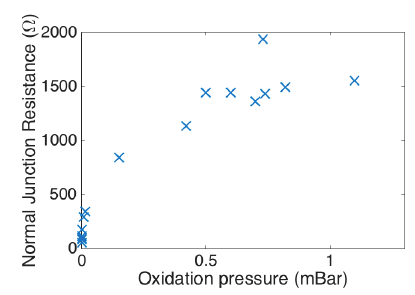
\includegraphics[height=4cm]{oxidation}
    \end{center}

  \item  BCS  theory  says  that  at zero  temperature,  there  is  a
    universal value
    \begin{equation}
      \Delta(0) = 1.73 \times  k_{b} \times T_{c},
    \end{equation}

    \noindent  that  depends  on  the  critical  temperature  of  the
    metal. For aluminium it is 1.3\,K.
  \end{itemize}
\end{framed}

\subsection{Quantising the Hamiltonian}
\subsubsection{\red{Charge energy dominates}, $ E_C/E_J >> 1$}
If charge  is the  important variable,  then we  chall work  with the
charge basis $ \lbrace N \rbrace $.  We use the number of phase operators derived
in \autoref{sec:charge_basis}.

\begin{framed}\noindent

  \begin{equation}
    \begin{aligned}
      e^{\pm i\hat{\blue{\phi}}} & = \sum_{n}\iketbra{n\pm 1}{n}\\
      \hat{\red{N}} & = \sum_{n}n\iketbra{n}{n}.
    \end{aligned}
  \end{equation}
\end{framed}

\noindent           and          exponentiating           \verb|cos|,
Eq.\eqref{eq:cooper-pair-box-summary} becomes

\begin{equation}
  \begin{aligned}
    \mathcal{H} & = 4E_C{\left(\hat{\red{N}}-N_\text{ext}\right)^2}- E_J\cos\left(\hat{\blue{\phi}}\right)\\
    & = 4E_C{\left(\hat{\red{N}}-N_\text{ext}\right)^2}- E_J \frac{1}{2}\left( e^{+i\hat{\blue{\phi}}} + e^{-i\hat{\blue{\phi}}} \right)\\
    &                                                               =
    \sum_n\bigg[4E_C{\left(n-N_\text{ext}\right)^2}\iketbra{n}{n}-
    \frac{E_J}{2}\bigg(\iketbra{n+1}{n}+\iketbra{n-1}{n}\bigg)\bigg]
  \end{aligned}.
  \label{l2-subbed2}
\end{equation}

\noindent which takes on the matrix form:
\begin{equation}\label{eq:cooper-pair-box-matrix-representation}
  \begin{pmatrix}
    4E_C(-2-N_\text{ext})^2 & -E_J/2 & 0 & 0 & 0\\
    -E_J/2 & \red{4E_C(-1-N_\text{ext})^2} & \red{-E_J/2} & 0 & 0\\
    0 & \red{-E_J/2} & \red{4E_C(N_\text{ext})^2} & -E_J/2 & 0\\
    0 & 0 & -E_J/2 & 4E_C(1-N_\text{ext})^2 & -E_J/2\\
    0 & 0& 0 & -E_J/2 & 4E_C(2-N_\text{ext})^2\\
  \end{pmatrix}
\end{equation}

\begin{figure}[h]
  \centering
  \includegraphics[height=7.5cm]{cooper-pair-box-as-a-function-of-next}
  \caption{\small    Plot   of    energies   and    ground-eigenstate
    contributions               -              taken               at
    $\Phi_{\text{ext}}=0$\label{fig:cp_box_energy_charge}}
\end{figure}

\noindent  In \autoref{fig:cp_box_energy_charge}  we demonstrate  the
energy  spectrum  and  contributions  of the  various  charge  states
(\iket{i}) to the ground state $ \Psi_g$:

\begin{equation}
  \iket{\Psi_{g}} = \sum_i^{\text{charge states}}\alpha_i \iket{i}.
\end{equation}

\begin{framed}\noindent
  The stronger the  coupling ($E_{J0}$) the greater  the splitting at
  the                        degeneracy                        points
  ($N_{\text{ext}} = \frac{2n + 1}{2}, n \in \mathbb{Z}$).
\end{framed}

\noindent  Furthermore, we  can run  the simulation  at a  fixed gate
charge   ($N_{\text{ext}}   =   0$)   but   varying   external   flux
($\Phi_{\text{ext}}$) (as done in an experiment in which we sweep the
field) - \autoref{fig:cooper-pair-box-as-a-function-of-phi-ext}.

\begin{figure}[h]
  \centering
  \includegraphics[height=7cm]{cooper-pair-box-as-a-function-of-phi-ext}
  \caption{\small  Fixed  charge  but  varied  flux  (what  we  would
    typically                                                     see
    experimentally).\label{fig:cooper-pair-box-as-a-function-of-phi-ext}}
\end{figure}

\subsection{Deriving energy from geometry}
\label{sec:back-transmon}

In               \autoref{fig:cp_box_energy_charge}               and
\autoref{fig:cooper-pair-box-as-a-function-of-phi-ext}  we hard-coded
in the  charging energy ($E_C=\iunit{70}{GHz}$) and  Josephson energy
($E_{J0}=\iunit{10}{GHz}$),                  but                 from
\autoref{eq:cooper-pair-box-summary} these  parameters are determined
by     the     geometry     of      the     qubit     depicted     in
\autoref{fig:cooper_pair_box_5_geometry}.

\begin{figure}[h]
  \centering \inkfig{12cm}{cooper_pair_box_5_geometry}
  \caption{\small     Energy      defined     by      geometry     of
    transmon\label{fig:cooper_pair_box_5_geometry}}
\end{figure}

Reading off the diagram
\begin{equation}
  \left\{
    \begin{aligned}
      E_c& = \frac{e^2}{2C_\Sigma}\\
      C_{\Sigma} & = \blue{C_\text{transmon} + C_g}+ \green{C_J}\\
      \blue{C_{g}} & = L_{g} \times 10^{-10}\\
      \blue{C_{\text{transmon}}} & = 4\times\left( L_{t} - 2S_{\text{transmon}} \right) \times 10^{-10}\\
      \green{C_J}   &    =   \frac{\varepsilon\varepsilon_0N_{sq}   \times
        A_{100\times100nm^2}}{d} \quad
      \text{where \iunit{d=2}{nm}, $\varepsilon = 10$}\\
      \red{E_{J0}} & = \frac{R_q}{R_{\square}/N_{sq}}\frac{\Delta(0)}{2}\\
      R_{\square} & = 1.84\,\text{k}\Omega \text{ for }100 \times 100\,\text{nm}^2 \qquad (1.5\,\text{k}\Omega \text{ at room temperature})\\
      \Delta(0)  &  =   1.73  \times  k_{b}  \times  T_{c}   \quad  \text{For  aluminium
        $T_{c}$ is \iunit{1.3}{K}}.
    \end{aligned}\right.
\end{equation}

\Autoref{fig:transmon-with-parameters-from-geometry} shows the energy
and transition spectrum for typical experimental geometry values.

\begin{figure}[h]
  \centering
  \includegraphics[height=7.5cm]{transmon-simulations/transmon-with-parameters-from-geometry}
  \caption{\small   Parameters    used:   $L_{g}   =    15\,\mu   m$,
    $L_{t}  =   150\mu  m$,   $2S_{\text{transmon}}  =   10\,\mu  m$,
    $N_{sq}=2$,     $d    =     \iunit{2}{nm}$,    $\varepsilon     =
    10$. \label{fig:transmon-with-parameters-from-geometry}}
\end{figure}

\subsubsection{Effect of $N_{\text{ext}}$ is negligible in transmon}
\label{sec:effect-n_textext}

The  ratio $E_{C}/E_{J0}<<0$  due  to the  shunting capacitance  that
suppresses the charging energy, meaning that charge will not strongly
affect the energy spectrum.  In \autoref{fig:cp_box_energy_charge} we
can  see  much flatter  (with  respect  to $N_{ext}$)  energies  when
$E_{J0}$ is much great than $E_C$.

This    can     be    confirmed,    by    varying     N$_{ext}$    in
\autoref{fig:transmon-sweep-N_ext}.

\begin{figure}[h]
  \centering
  \includegraphics[height=6cm]{transmon-simulations/transmon-sweep-N_ext}
  \caption{\small      Sweeping     the      gate-induced     charge,
    $N_{\text{ext}} = \frac{V_{g}C_{g}}{2e}$ has little effect on the
    energy of the system, since  any variations are suppressed by the
    big shunting capacitance. \label{fig:transmon-sweep-N_ext}}
\end{figure}

\subsubsection{Using   sufficient  number   of   charge  states   for
  simulation}
\label{sec:note-simulation}

It is always best to utilise as many charge states for a simulation -
convergence                occurs                as                in
\autoref{fig:transmon-sweep-number-of-charge-states}.

\begin{figure}[h]
  \centering
  \includegraphics[height=13cm]{transmon-simulations/transmon-sweep-number-of-charge-states}
  \caption{\small  Including more  charge  states  in the  simulation
    results  in  a more  accurate  simulation  -  at some  point  the
    energies stop  changing, at  which point  the simulation  is good
    enough.\label{fig:transmon-sweep-number-of-charge-states}}
\end{figure}

\subsubsection{Maintaining anharmonicity}
\label{sec:maint-anharm}

The robustness to charge noise,  that is always present in electrical
systems, demonstrated in  \autoref{sec:effect-n_textext} is countered
by the vanishing assymetry between the transitions

\begin{equation}\label{eq:transmon-assymetry}
  \alpha = \frac{E_{21} - E_{10}}{E_{10}}.
\end{equation}

\noindent  Increasing  $E_J/E_C$  will  lead  to  the  domination  of
$\cos\left(\hat{\blue{\phi}}\right)$                               in
$E_C{\left(\hat{\red{N}}-N_\text{ext}\right)^2}-
E_J\cos\left(\hat{\blue{\phi}}\right)$. The  state of the  system can
be viewed as a particle in a periodic potential, becoming exceedingly
localised  in  the  potential minima.   \red{Insert  derivation  from
  Bader}.

\noindent  Just compare  the  anharmonicity for  different values  of
$E_C$ in \autoref{fig:transmon-anharmonicity}.

\begin{figure}[h]
  \centering
  \includegraphics[height=9cm]{transmon-simulations/transmon-anharmonicity}
  \caption{\small         Anharmonicity         vanishes         when
    $E_{C}/E_{J0} << 1$\label{fig:transmon-anharmonicity}}
\end{figure}

\subsection{Charge dispersion}
\label{sec:charge-dispersion}

The  transmon  must be  robust  against  charge variations  (maximise
$E_J/E_C$) so that charge variations in the circuit do not affect the
energy levels. \red{Bader derivation} goes through how deep decoupled
states in  the well it  is best to assume  that the energy  levels of
individual  wells are  known,  but coupling  between these  ``wells''
perturbs the initial energies.

\begin{figure}[h]
  \centering \inkfig{8cm}{wavefunction_transmon}
  \caption{\small View system as a  particle in a periodic potential.
    It has very little Kinetic energy, so it will be localised in the
    minima.\label{fig:wavefunction_transmon}}
\end{figure}

The wavefunction is suppressed by  the potential barrier.  The higher
the  relative size  of the  barrier (high  $E_J/E_C$) the  higher the
decoupling and the less

\subsection{Summary for transmon}
\label{sec:summary-transmon}

\begin{figure}[h]
  \centering
  \includegraphics[height=12cm]{2020-09-05_(cooper-pair-box-and-transmon)/transmon-anharmonicity-and-charge-dispersion}
  \caption{\small  We want  to  maximise  the anharmonicity  $\alpha$
    (have it in  the blue region) and minimise  sensitivity to charge
    ($\varepsilon_m         =        \frac{E_m(N_{ext}=0.5)         -
      E_m(N_{ext}=0)}{E_{10}}$) (green region).   This is achieved by
    having  $5 \le  E_{J0}/E_C \le  70$ We  need to  use many  charge
    states in order to get a good approximation (50 used here, and it
    is                 still                  only                 an
    approximation)\label{fig:transmon-anharmonicity-and-charge-dispersion}}
\end{figure}

The addition  of a shunt capacitance,  $C_{\text{transmon}}$, reduces
$E_{C}$ -  energy associated  with the capacitance  circuit elements,
which  has  two counter-opposing  effects  that  are demonstrated  in
\autoref{fig:transmon-anharmonicity-and-charge-dispersion}
\begin{itemize}
\item Robustness of the system against charge noise, which occurs for
  $\mathbf{E_{J0}/E_C>5}$ \hfill \autoref{sec:effect-n_textext};
\item  Vanishing   of  the  anharmonicity  required   for  addressing
  individual transitions - \red{\textbf{the anharmonicity needs to be
      at least larger than the  spectrum width of the 0-1 transition.
      This will  typically be 200MHz,  meaning that for a  spacing of
      \iunit{5-20}{GHz}   one    will   need   $\alpha    >   0.04$}}
  \cite{Kjaergaard_2020} \hfill \autoref{sec:maint-anharm}.

  Now as per  \autoref{tab:conversion2}, increasing $C_{transmon}$ is
  equivalent to a particle in the  potential acquiring more mass - it
  becomes localised in one of the  potential minima, in which case we
  approximate  cosine with  a parabollic  potential and  according to
  \cite{Koch_2007} find that

\begin{equation}\label{eq:transmon-anharmonicity}
  \alpha = \frac{-E_{C}}{\omega_{10}} = -\frac{1}{\sqrt{8E_{J0}/E_C} - 1} \quad \Rightarrow \quad \frac{E_{J0}}{E_C} = \frac{1}{8}\left( 1 - \frac{1}{\alpha} \right)^2,
\end{equation}

\noindent so for $\alpha>0.04$ one would need $E_{J0}/E_C < 70$:
\end{itemize}

\begin{framed}\noindent
  \noindent We need to find  a compromise that fulfills the following
  criteria:

  \begin{itemize}
  \item  Maintain  anharmonicity  $\iabs{\alpha} \ge  0.04  $  \hfill
    \red{$E_{J0}/E_C < 70$};
  \item Reduce the charge  dispersion $\varepsilon_m < 0.0001$ \hfill
    \red{$E_{J0}/E_C > 5$};
  \item We  need the transition energy  to be within the  window that
    our     laboratory     equipment      can     register     \hfill
    \red{\iunit{5-20}{GHz}};
  \end{itemize}
\end{framed}

\subsubsection{Choosing ratio}
Let  us choose  $E_C$  and  $E_{J0}$ to  fulfil  the above  criteria.
Hard-coding               some               values,               in
\autoref{fig:transmon-optimal-parameters},  we  get  a  selection  of
$E_C$ and $E_{J0}$  energies to use, which  we will keep a  log of in
\autoref{tab:transmon-fabrication-parameters}.    In  order   to  use
consistent  cross  sizes  (simpler  to   draw)  we  will  choose  the
$E_C=1GHz$ for a transmon length of $L_{\text{transmon}}$

\begin{figure}[h]
  \centering
  \includegraphics[height=4cm]{2020-09-05_(cooper-pair-box-and-transmon)/selecting-EJ0-to-fall-in-range_EC=5GHz}%
  \includegraphics[height=4cm]{2020-09-05_(cooper-pair-box-and-transmon)/selecting-EJ0-to-fall-in-range_EC=2GHz}%
  \includegraphics[height=4cm]{2020-09-05_(cooper-pair-box-and-transmon)/selecting-EJ0-to-fall-in-range_EC=1GHz}%
  \caption{\small Optimal parameters for  transmon.  Left to right we
    increase $E_C$  and within each  plot display values  for varying
    $E_{J0}$, Red  region shows  the window  of devies.   Solid lines
    show  $\alpha \ge  0.04$.   We will  choose  the bigger  transmon
    (suppressing $E_C$) as it allows  for a broader range of $E_{J0}$
    values.\label{fig:transmon-optimal-parameters}}
\end{figure}

\begin{framed}\noindent
  $\blue{E_C(L_{\text{transmon}})}$ and  $\red{E_{J0}(N_{sq})}$ where
  the calibration curves  are given in \autoref{fig:EJ0-EC-selection}
  - this completes \autoref{tab:transmon-fabrication-parameters}.
  \begin{equation}
    \left\{
      \begin{aligned}
        L_\text{gate} & = 15\mum\\
        C_{\text{gate}} & = L_\text{gate} \times 10^{-10} = \iunit{1.5}{fF} - \text{negligible}\\
        2S_{\text{transmon}} & = 10\mum \\
        \blue{C_{\text{transmon}}} & = 4\times\left( L_{\text{transmon}} - 2S_{\text{transmon}} \right) \times 10^{-10} \\
        A_{JJ} &  = N_{sq} \times 100\times100nm^{2} \\
        C_J & = \frac{\varepsilon\varepsilon_0A_{JJ}}{d} \quad \text{
          \iunit{d=2}{nm}, $\varepsilon = 10$}\\
        C_{\Sigma} & = \blue{C_\text{transmon}} + C_g + C_J \approx \blue{C_\text{transmon}}\\
        E_c& = \frac{e^2}{2C_\Sigma}\\
        \red{E_{J0}} & = \frac{R_q}{R_{\square}/\red{N_{sq}}}\frac{\Delta(0)}{2} \quad R_q=6.43\kOhm \quad R_{\square} = 1.84\kOhm \text{ for } 100 \times 100\,\text{nm}^2\\
      \end{aligned}\right.
  \end{equation}
\end{framed}

\begin{figure}[h]
  \centering%
  \includegraphics[height=6cm]{2020-09-05_(cooper-pair-box-and-transmon)/EJ0-selection}%
  \includegraphics[height=6cm]{2020-09-05_(cooper-pair-box-and-transmon)/EC-selection}
  \caption{\small More JJ squares  mean smaller resistance and higher
    critical current $\Rightarrow  E_{J0}$ increases.  Large transmon
    size   means  less   charge  concentration   $\Rightarrow  E_{C}$
    decreases.                                                      @
    $E_C(L_{\text{transmon}}=350)                                   =
    0.59\,$GHz\label{fig:EJ0-EC-selection}}
\end{figure}

 \begin{table}[h]
   \centering
   \caption{Example     $E_C$     and     $E_{J0}$     values     for
     fabrication. $2S_{\text{transmon}}=24\mum$ \label{tab:transmon-fabrication-parameters}}
   \begin{tabular}{|c|c|c|c|c|c|c|}
     \hline
     $E_{C}$ (GHz) & $E_{J0}$ (GHz) & Ratio &  $L_{\text{transmon}} (\mum)$ & $N_{sq}$ & Square side (nm) & Resistance/RT (k$\Omega$)\\\hline
     0.85 &               10 &    11.8 &              251 &                  0.12 &              34.6 &                    15.33/12.50  \\
     0.85 &               17 &    20.0 &              251 &                  0.21 &              45.8 &                    9.67/7.89  \\
     0.85 &               40 &    47.1 &              251 &                  0.49 &               70. &                    3.75/3.06     \\
     0.85 &               80 &    94.1 &              251 &                  0.97 &              98.5 &                    1.90/1.55  \\
     1 &               20 &    20.0 &              217 &                  0.24 &              49.0 &                    7.67/6.25  \\
     0.6 &              100 &   166.7 &              345 &                  1.22 &              110. &                    1.508/1.23 \\
     0.6 &              120 &   200.0 &              345 &                  1.46 &              121. &                    1.26/1.03 \\\hline
   \end{tabular}
 \end{table}

 \noindent An  example of the  resulting structure is given  in table
 \autoref{tab:transmon-fabrication-parameters}.

 \begin{figure}[h]
   \centering
   \includegraphics[width=0.3\textwidth]{2020-09-22_teresa_xmon/2020-09-22_teresa_xmon-1}
   \includegraphics[width=0.3\textwidth]{2020-09-22_teresa_xmon/2020-09-22_teresa_xmon-2}
   \includegraphics[width=0.3\textwidth]{2020-09-22_teresa_xmon/2020-09-22_teresa_xmon-3}
 \end{figure}

 \noindent


 \newpage
 \subsection{Transmon 2-level approximation}
 \label{sec:transmon-2-level}


 \noindent  Normally $  N_\text{ext}  $  is biased  at  a sweet  spot
 \red{close to $ -  1/2 $}. Then the only number  of electrons $n$ on
 out island that will give a low energy (due to the energy dispersion
 in  Fig.~\ref{fig:cp_box_energy_charge}) is  either  0  or -1.   The
 other level will be far separated. Then we take out the Hamiltonian

 \red{\begin{equation}
     \begin{aligned}
       \mathcal{H}_\text{0 or -1} & = \begin{pmatrix}
         E_C(-1-N_\text{ext})^2 & -E_J/2\\
         -E_J/2 & E_C(N_\text{ext})^2\\
       \end{pmatrix}\\
     \end{aligned}
   \end{equation}}

 \noindent And  we have a  two level system  just as in  the previous
 lecture Eq.\eqref{l1-finalEVal}.   Redefining the zero  point energy
 to be in the middle of the diagonal terms

 \begin{equation}
   \begin{aligned}
     \mathcal{H} & = \begin{pmatrix}
       -\epsilon/2 & -E_J/2\\
       -E_J/2 & \epsilon/2\\
     \end{pmatrix}\\
     \epsilon/2     =     \frac{\text{energy    diff}}{2}     &     =
     \frac{E_CN_\text{ext}^2-E_C(1+N_\text{ext})^2}{2}              =
     -\frac{E_C}{2}\big(1+2N_\text{ext}\big)
   \end{aligned}
 \end{equation}

\begin{framed}\noindent
  This will have solutions

   \begin{equation}
     E = \pm \frac{\Delta E}{2}, \qquad \ket{\psi}_0 = \begin{pmatrix}
       \cos(\theta/2) \\ \sin(\theta/2)
     \end{pmatrix},  \qquad  \ket{\psi}_1  = \begin{pmatrix}  \sin(\theta/2)  \\
       \cos(\theta/2)
     \end{pmatrix}, \Delta E = \sqrt{\epsilon^2+\Delta^2}
   \end{equation}
 \end{framed}

 \begin{itemize}
 \item In Fig.\ref{l3-energyspec} depicted  are the energy levels for
   different  values  of the  charging  and  coupling energies.   The
   stronger the  coupling, $ E_J $,  the bigger the splitting  at the
   degeneracy points.

   \red{There  is   less  charge   noise  in   the  sweet   spots  of
     $ n_g  = \mathbb{Z}\frac{1}{2} $, but  it will still be  a major
     source  of decoherence.   \textbf{There  is  less dependence  on
       charge fluctuations as  $ E_C/E_J $ gets smaller  and the band
       become flatter}.}
   \begin{figure}[h]
     \centering 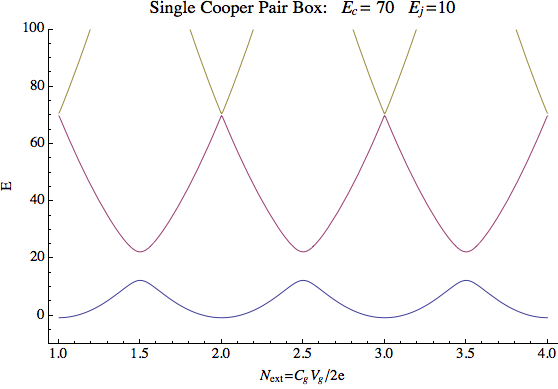
\includegraphics[height=6cm]{cpb2}
   \end{figure}

\noindent
different  at   the  degeneracy  point  grows   as  coupling  becomes
stronger.\label{l3-energyspec}

\item One can also looks the  ground energy state (the one the system
  will most probably occupy) and find the components that make it up

  \[
    \Ket{\Psi}_{\text{ground}} = \sum_N\alpha_N\ket{N},
  \]

  \noindent and one sees in the figures when there is no applied gate
  voltage,   the  island   will  have   $   N=0  $   charges  on   it
  predominantly. As  one increases the  gate charge, the  presence of
  $ N=1 $ increases, until it finally dominates.  The pattern repeats
  as more  and more cooper  pairs tunnel,  to give the  lowest energy
  configuration.
\end{itemize}

\begin{framed}\noindent
  \textbf{High $ E_C/E_J $:}
  \begin{itemize}
  \item High charge noise -  gate voltage changes, affects the energy
    levels severely
  \item High  anharmonicity - quadratic  $ n $  dependance dominates,
    allowing individual addressing of the levels;
  \end{itemize}

\end{framed}

\newpage\subsubsection{\red{Flux energy dominates, $ E_C/E_J << 1 $}}
If flux is  the important variable, then we chall  work with the flux
basis using the wavefunctions $ \psi(\phi) $

\begin{framed}\noindent

  \begin{equation}
    \begin{aligned}
      &\blue{\hat{\phi}} \qquad\\
      &\red{\hat{N}} = -i\frac{d}{d\blue{\phi}}
    \end{aligned}
  \end{equation}

\end{framed}
\noindent and we rewrite

\begin{equation}
  \begin{aligned}
    \mathcal{H} & = E_C{\left(\hat{\red{N}}-N_\text{ext}\right)^2}- E_J\cos\left(\hat{\blue{\phi}}\right)\\
    & = E_C\left(-i\frac{d}{d\phi} - n_g\right)^2 - E_J\cos(\phi).
  \end{aligned}
\end{equation}

\begin{itemize}
\item Let us compare this to Hamiltonian in a periodic potential
  \begin{equation}
    \mathcal{H}_\text{crystal} = \frac{-\hbar^2}{2m}\frac{d^2}{dx^2}+V(x)\qquad V(x+a) = V(x),
  \end{equation}

  \noindent  which, according  to  Bloch's theorem,  states that  the
  eigenstates will be of the form
  \begin{equation}
    \psi_{kn}(x) = e^{ikx}u_{kn}(x),
  \end{equation}
  \noindent  which,  when plugged  in  will  result in  an  effective
  Hamiltonian

  \begin{equation}
    \mathcal{H}_{\text{eff},k} = \frac{\hbar^2}{2m}\left(-i\frac{d}{dx}+k\right)^2 + V(x)
  \end{equation}
\item We can see this mapping between
  \begin{equation}
    \begin{aligned}
      \mathcal{H}_{\text{eff},k} & = \frac{\hbar^2}{2m}\left(-i\frac{d}{dx}+k\right)^2 + V(x)\\
      \mathcal{H}  & =  E_C\left(-i\frac{d}{d\phi}  - n_g\right)^2  -
      E_J\cos(\phi),
    \end{aligned}
  \end{equation}

  \noindent so, will look for solutions of a similar form.
\item  As $  E_C/E_J  $ gets  smaller, the  potential  well from  the
  $ E_J\cos(\phi) $ gets deeper  \red{\textbf{and the states within each
      well  localise,  and  stop   interacting  with  one  another.}}
  Solving,  as in  the  Transmon Paper,  will  lead to  anharmonicity
  relation

  \begin{framed}\noindent
    \begin{equation}       \frac{E_{12}      -       E_{01}}{E_{01}}\approx
      -(8E_J/E_C)^{-1/2},
    \end{equation}
    \noindent which decreases as we continue to increase $ E_J $.
  \end{framed}
\end{itemize}
\newpage

%%% Local Variables:
%%% mode: latex
%%% TeX-master: "all_the_notes"
%%% End:
